\documentclass{article}
\usepackage{nips15submit_e,times}
\usepackage{amssymb}
\usepackage{tikz}
\usepackage{neuralnetwork}

\title{Learning To Evaluate Arimaa Positions}

\author{
Alan J. Zaffetti\thanks{B.S. Computer Science} \\
College of Information and Computer Sciences\\
University of Massachusetts Amherst\\
Amherst, MA 01003 \\
\texttt{azaffett@umass.edu} \\
}

\begin{document}
\maketitle
\begin{abstract}
Arimaa is a two-player abstract strategy game.  A chess variant, it was designed to be computer-resistant, since each position has a combinatorial number of moves.  Last year, however, David Wu showed that this computer-resistance was limited, developing a bot which beat top human players \cite{wu}.  In this paper, we examine a regression problem: learning a function to evaluate the winning chances in Arimaa positions.  To solve it, we propose a 3-layer convolutional neural network.  If successful, the model will serve as a useful heuristic to further playing strength.
\end{abstract}

\section{Introduction}

\subsection{On Arimaa}

\begin{figure}[ht]
\centering
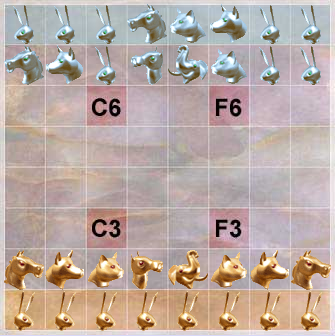
\includegraphics[scale=.4]{assets/example.png}
\caption{The players begin a game by setting up their pieces however they choose on their home rows.  There is no standard initial configuration for Arimaa.}
\end{figure}

Arimaa was developed in 2002 by Omar Syed, who was inspired by the 1997 IBM Deep Blue match versus Gary Kasparov to create a more computer-resistant chess variant.  The game is computer-resistant because it has a combinatorial number of moves in every position.  Players can make between 1-4 steps per turn, and may spend those steps on any combination of legal pieces.  After eliminating steps that result in the same position, on average there are about 17,000 legal moves per turn \cite{haskin}.  Compare this to Go, which has, on average, 250.  Dispite this major hinderance to search, intrisic properties of the game, and the addition of sophisticated heuristics borrowed from the computer chess literature, and tuned over many years, have helped reduce the effective branching factor thousands of times \cite{wu}.

\subsection{On CNN}

Convolutional neural networks (CNN) have seen great success in late applications to machine learning, particularly computer vision, and image processing tasks.  They are characterized by layers of learnable filters (or kernels), which are convolved across the input image (computing a dot product between the two).  The result are filters which activate when they see some specific type of feature.  

\section{Related Work}

Oshri and Khandwala \cite{Oshri_Khandwala} is a relevant work on training a CNN to predict chess moves.  Although the problem domain differs, many of the methods and data structures used are relevant for us.  For example, we use their method for encoding the $8\times 8$ chess board in 6 channels.  We also take some of their findings on CNN architecture in to consideration.

Google DeepMind's recent victory of AlphaGo versus Lee Sedol has shown that games are still not exempt from this heyday.  Given appropriate architectures, valid datasets, and increasingly massive computational resources, these approaches challenge human's experienced-based reasoning, especially under the closed conditions of a game board.

The success of CNN-Go, generally, can be attributed to the smooth arrangements of positions that are approximately continuous through and between games \cite{Oshri_Khandwala}.  In Go, only one piece is placed per turn.  Since pieces are not allowed to move, the inherent entropy of the game is lessened dispite a large branching factor.  Arimaa shares a weaker version of this property.  Although, pieces can move, each piece moves in the same way, namely one space at a time in cardinal directions.  We predict the resultant spacial relationships will be easier to encode than in chess, for instance.  For this reason, we expect that CNN-Arimaa will have similar success.

\section{Data Set}
Arimaa.com game room offers an archive of all games played on their servers \cite{arimaa_com}\cite{games}.  I process a subset of this data (minimum ELO rating 1800 and above) amounting to 46210 expert games.  From these games, I extracted a number of key positions (maximum of 160 plys beginning from the end of the game.)  This is a more-than-sufficient sample rate, since the average Arimaa game is only 100 plys.  This last processing step gave me the final dataset of 3,977,256 positions as datacases containing, in total, 1,527,266,304 features.  For each datacase, there are 384 features and 1 label corresponding to the backpropogated game result from the game which produced it.  Ties are not possible in Arimaa, so the only possible labels are ``will the side to move win?'' (1) or ``will the side to move lose?'' (0).  Only games that resulted in a meaningful win were used.

\subsection{Feature Encoding}
After filtering the list of expert games, position data was obtained by taking the provided lists of moves, playing them out to the end, then popping off the last 160 plys and recording them.  Thus, the lists of moves are turned into  $8\times 8$ board states.  The resultant board data is split into 6 channels (one for each piece) producing $6\times 8\times 8$ \textit{bitboard} matrices.  We implement seperate channels because piece values are not continouosly comparable, and therefore cannot be represented on the same channel.  Pieces for the side to move use a 1, the opposing side uses -1, and empty squares are 0.  This can be viewed as a form of dimensionality reduction, since the same representation can predict a board of gold to move, or conversely, a board with silver to move, where all symmetries have been eliminated.

\section{Proposed Solution}

\subsection{CNN Architecture}

The proposed model is a 3-layer neural network with 384 inputs and a single output.  The proposed network architecture is one level of convolution, a single hidden layer, and a rectified output layer.  Initially, the convolutional layer uses 384 square $3\times3$ kernels.  The inner hidden layer is comprised of 384 units.  Both the convolutional layer and hidden layers use $tanh$ as their activation functions.  During experiments, we found this function worked best.  The output layer uses a rectified linear activation function to fit the regression problem.

\begin{figure}[ht]
\centering
\begin{neuralnetwork}[height=4]
	\newcommand{\nodetexty}[2]{$y_#2$}
	\newcommand{\mynodetext}[2]{$\vdots$}
	\setdefaultnodetext{\mynodetext}
	\inputlayer[count=3, bias=true, title=Input\\layer, text=\mynodetext]
	\hiddenlayer[count=3, bias=true, title=$tanh$\\conv layer, text=\mynodetext] \linklayers
	\hiddenlayer[count=3, bias=true, title=$tanh$\\layer, text=\mynodetext] \linklayers
	\outputlayer[count=1, title=Rectified\\output, text=\nodetexty] \linklayers
\end{neuralnetwork}
\caption{A sample of the neural network architecture with included bias terms (top).  Not all terms are shown.}
\end{figure}

We chose to keep the CNN architecture fixed and relatively small, because, as we found, training and validating larger networks is increasingly impossible, save for increasing the batch size.  With 48 learnable filters, and 384 hidden units, we claim our proposed network has sufficient capacity for our purposes that we do not consider deeper architectures.

We used the scikit-neuralnetwork (sknn) package for training the CNN, which is a friendly wrapper over pylearn2, which itself is built over Theano \cite{theano}.

\subsection{Validation}

We cannot afford to do validation over all 3.9 million examples, therefore, we limited our validation experiments down to a smaller number of examples for each parameter setting in the joint parameter space.  We experimented with different learning rules, regularizers, layer normalization methods, convolution kernel shapes, and dropout rates.  $K$-fold cross-validated grid-search is used to determine the effectiveness of the measures and which combination worked best.

\subsection{Training}

The optimal hyperparameters found during validation are used to train a network on the full dataset.  The batch size is increased from 16 to 4096 to accomadate the larger number of instances.  We shuffle the full dataset before using it since the timeseries bias could negatively effect the learning rate.

\section{Experiments}

\subsection{Cross-Validated Grid Search}

30000 shuffled examples are selected from a larger pool of 1.8 million examples to prevent overfitting.  We find optimal hyperparameters using a 2-fold cross-validated grid-search over these micro-datasets.  Batch size is set to 1000 to expedite the search; MSE loss is used.  We expect optimal parameters to fit the larger dataset, since they were tested on samples from the target distribution.

\begin{figure}[ht]
\centering
\begin{tabular}{|l|l|}
\hline
\textbf{Parameter} & \textbf{Tested Values} \\
\hline
\textit{Dropout Rate} &  .5, .25, .1, .05, .01, .005, None \\
\textit{Regularization} &  L1, L2, None \\
\textit{Learning Rule} & sgd, rmsprop, momentum, nesterov \\
\textit{Kernel Shape} & $(2\times 2)$, $(3\times 3)$, $(4\times 4)$, $(5\times 5)$, $(6\times 6)$, $(1\times 4)$, $(1\times 8)$, $(3\times 1)$, $(6\times 1)$ \\
\hline
\end{tabular}
\caption{The space of parameters we cross-validated.}
\end{figure}

Initially, we experiment with $6\times 6$ kernels to narrow the space of parameters.  Our results for this stage were used to find our final optimal hyperparameters, which we present in Figure \ref{fig:paramtable}.

\begin{figure}[ht]
\centering
\begin{tabular}{|l|l|l|l|l|l|l|l|}
\hline
\textbf{MSE} & \textbf{MAE} & \textbf{$R^2$} & \textbf{Acc\footnote{Accuracy was obtained by rounding $\textbf{y}^\prime$ to the nearest whole number.  When rounded, outputs can be interpreted as a binary classification.}} & \textbf{Dropout} & \textbf{Regularizer} & \textbf{Learning Rule} & \textbf{Kernel Shape} \\
\hline
.0803 & .1870 & .6787 & .899 & None & L1 & nesterov & $4\times 4$ \\
.0804 & .1868 & .6785 & .899 & None & L2 & nesterov & $4\times 4$ \\
.0804 & .1867 & .6785 & .8991 & None & None & nesterov & $4\times 4$ \\
.0833 & .1917 & .6670 & .8938 & .01 & L1 & nesterov & $4\times 4$ \\
.0833 & .1918 & .6669 & .8939 & .005 & L1 & nesterov & $4\times 4$ \\
.0833 & .1916 & .6668 & .8935 & .01 & None & nesterov & $4\times 4$ \\
.0833 & .1917 & .6667 & .8939 & .005 & L2 & nesterov & $4\times 4$ \\
.0833 & .1917 & .6667 & .8939 & .005 & None & nesterov & $4\times 4$ \\
\hline
\end{tabular}
\caption{Our results show a clear preference for Nesterov momentum (over SGD\footnote{stochastic gradient descent}), which dominated the top spots in our experiments.  Regularization has had some positive impact.  This is consistant with Oshri and Khandwala, who posited that a small amount of regularization might be applicable to their chess network model \cite{Oshri_Khandwala}. Our results show L1 regularizer improves $R^2$ and MSE.  Dropout was detrimental to model fitting.  This is consistant with Oshri and Khandwala, who claim the image was small enough that all features must be interacting with eachother \cite{Oshri_Khandwala}. \label{fig:paramtable}}
\end{figure}

\section{Results}

We ran the optimal hyperparameters on the full dataset, training the network for 30 iterations.  The batch processing size was increased to 4096 to accomadate the large number of examples.  We set aside $1/5$ of the data for held-out test data; we could not to do full cross-validation on the model since it already took over an hour to train.  After 30 iterations, the final result for our model was achieved: MSE=$.171$, with a classification accuracy of $73.5\%$ predicting the outcome of games from positional features alone.  Figure \ref{fig:hplot} shows a detailed plot of our results against the original set of games.

\begin{figure}[ht]
\centering
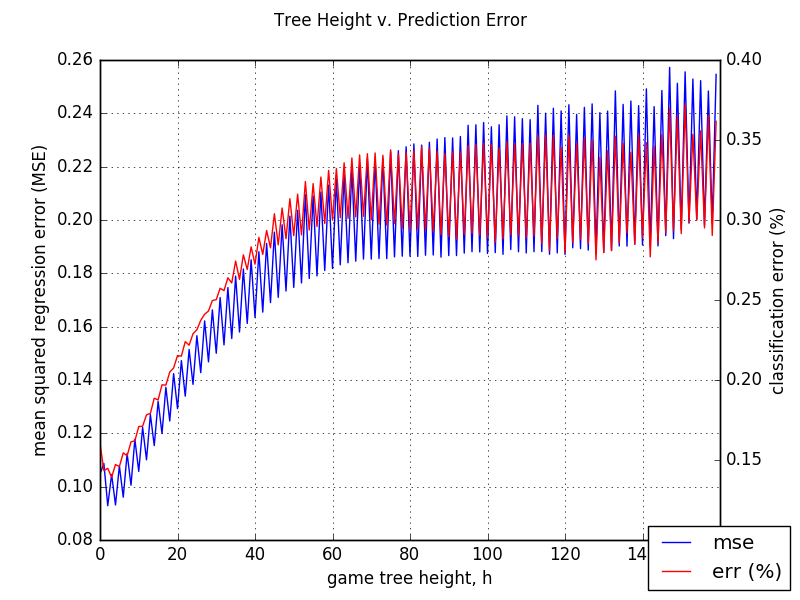
\includegraphics[scale=.5]{assets/figure-hplot.png}
\caption{The model's regression error is the lower line shown in blue.  $0/1$-classification error is also included above it (red).  This ``height plot'' elucidates our models predictive power at varying heights in the game tree.  In the end game ($h=0$) our model has MSE $.105$ and classification error $15\%$.  MSE seems to rise up through middlegame, with a peak at the opening (MSE=$.22\pm .02$), while classification error plateus and holds at the point of maximum entropy near the middlegame (error=$32.5\pm 3 \%$). \label{fig:hplot}}
\end{figure}

\subsection{Convolutional Filters}

\begin{figure}[h]
\centering
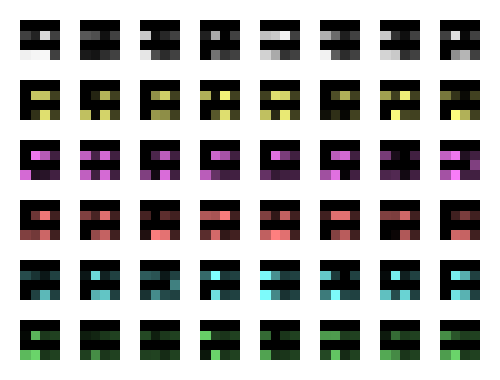
\includegraphics[scale=.5]{assets/figure-filters.png}
\caption{Colorized $4\times 4$ convolutional filters as learnt by our model.  Each row corresponds to a distinct channel, one for each piece.  From top to bottom: rabbit (white), cat (yellow), dog (pink), horse (red), camel (cyan), and elephant (green). }
\end{figure}

\section{Discussion}

\begin{itemize}
\item \textbf{Reinforcement Learning} Given more time, we would have definitely wanted to explore the area of using self play as a form of reinforcement learning.  Given a set of strong base models, we implement self-play by pitting pairs of models against oneanother in rounds of rapid Monte Carlo style games.  Self-play would be crutial in developing an actual top-level Arimaa bot.

\item \textbf{Pipeline Improvements} The data scale caused each stage of the pipeline to take a while to run:  1-2 hours to compile the data, 1 hour to select hyperparameters, and 1 hour train the model.  All of these stages are embarressingly parallel, but no effort was devoted to writing the parallel code.  Languages such as Spark \cite{spark} and hosted environments such as AWS EC2 could have helped expedited the pipeline enormously.

\item \textbf{Reevaluate `Meaningful Games'} Included in our dataset are games that ended in resignation (one player gives up).  We conjecture that including these games has increased the error near the tail-end of our predictions in Figure \ref{fig:hplot}, because an early resignation does not always look like a goal.  Given more time, we would purge these data-cases and attempt to re-train.

\item \textbf{More Robust Parameter Selection} Given more time, I would have liked to perform more hyperparameter selection using larger datasets, particularly for learning rates and pooling.
\end{itemize}

\section{Conclusion}

In this paper, we examined a regression problem: learning a function to evaluate the winning chances in Arimaa positions.  We proposed a 3-layer convolutional neural network: one layer of convolution filters, one hidden layer, and a rectified output layer.  In the end, our model was able to predict winning chances with an squared error margin of $0.171$, and predicted the correct outcome of games $73.5\%$ of the time.  The predictions were made using positional features alone from a set of 46210 expert Arimaa games.

\begin{thebibliography}{9}

\bibitem{arimaa_com}
Arimaa Gameroom;
\textit{http://arimaa.com};
2002-2016.

\bibitem{haskin}
Haskin, B. (2006). A Look at the Arimaa Branching Factor. http://arimaa.janzert.com/bf study/. Accessed on 2015-07-12.

\bibitem{games}
Arimaa Games Archive;
\textit{http://arimaa.com/arimaa};
2002-2016.

\bibitem{puzzles}
Arimaa `Win in 2' puzzles;
\textit{http://arimaa.com/arimaa};
2002-2016.

\bibitem{fen}
Forsyth--Edwards Notation;
\textit{https://en.wikipedia.org/wiki/};
2016.

\bibitem{spark}
Apache Spark;
\textit{https://spark.apache.org};
2016.

\bibitem{theano}
Theano;
\textit{http://deeplearning.net/software/theano/};
2016.

\bibitem{nolearn_lasagne}
Nolearn.lasagne;
\textit{https://pythonhosted.org/nolearn/lasagne.html}
2016.

\bibitem{wu}
Wu, David J. (March 2015).
Designing a Winning Arimaa Program.
ICGA Journal.

\bibitem{Hrebejk}
Hrebejk, T. (2013). Arimaa challenge - static evaluation function. M.Sc. thesis, Charles University, Prague.

\bibitem{Oshri_Khandwala}
Oshri, Barak. Khandwala, Nishith. (2015).  Predicting Moves in Chess using Convolutional Neural Networks.  Stanford University.

\end{thebibliography}

\end{document}